\begin{figure*}[t]
  \centering
  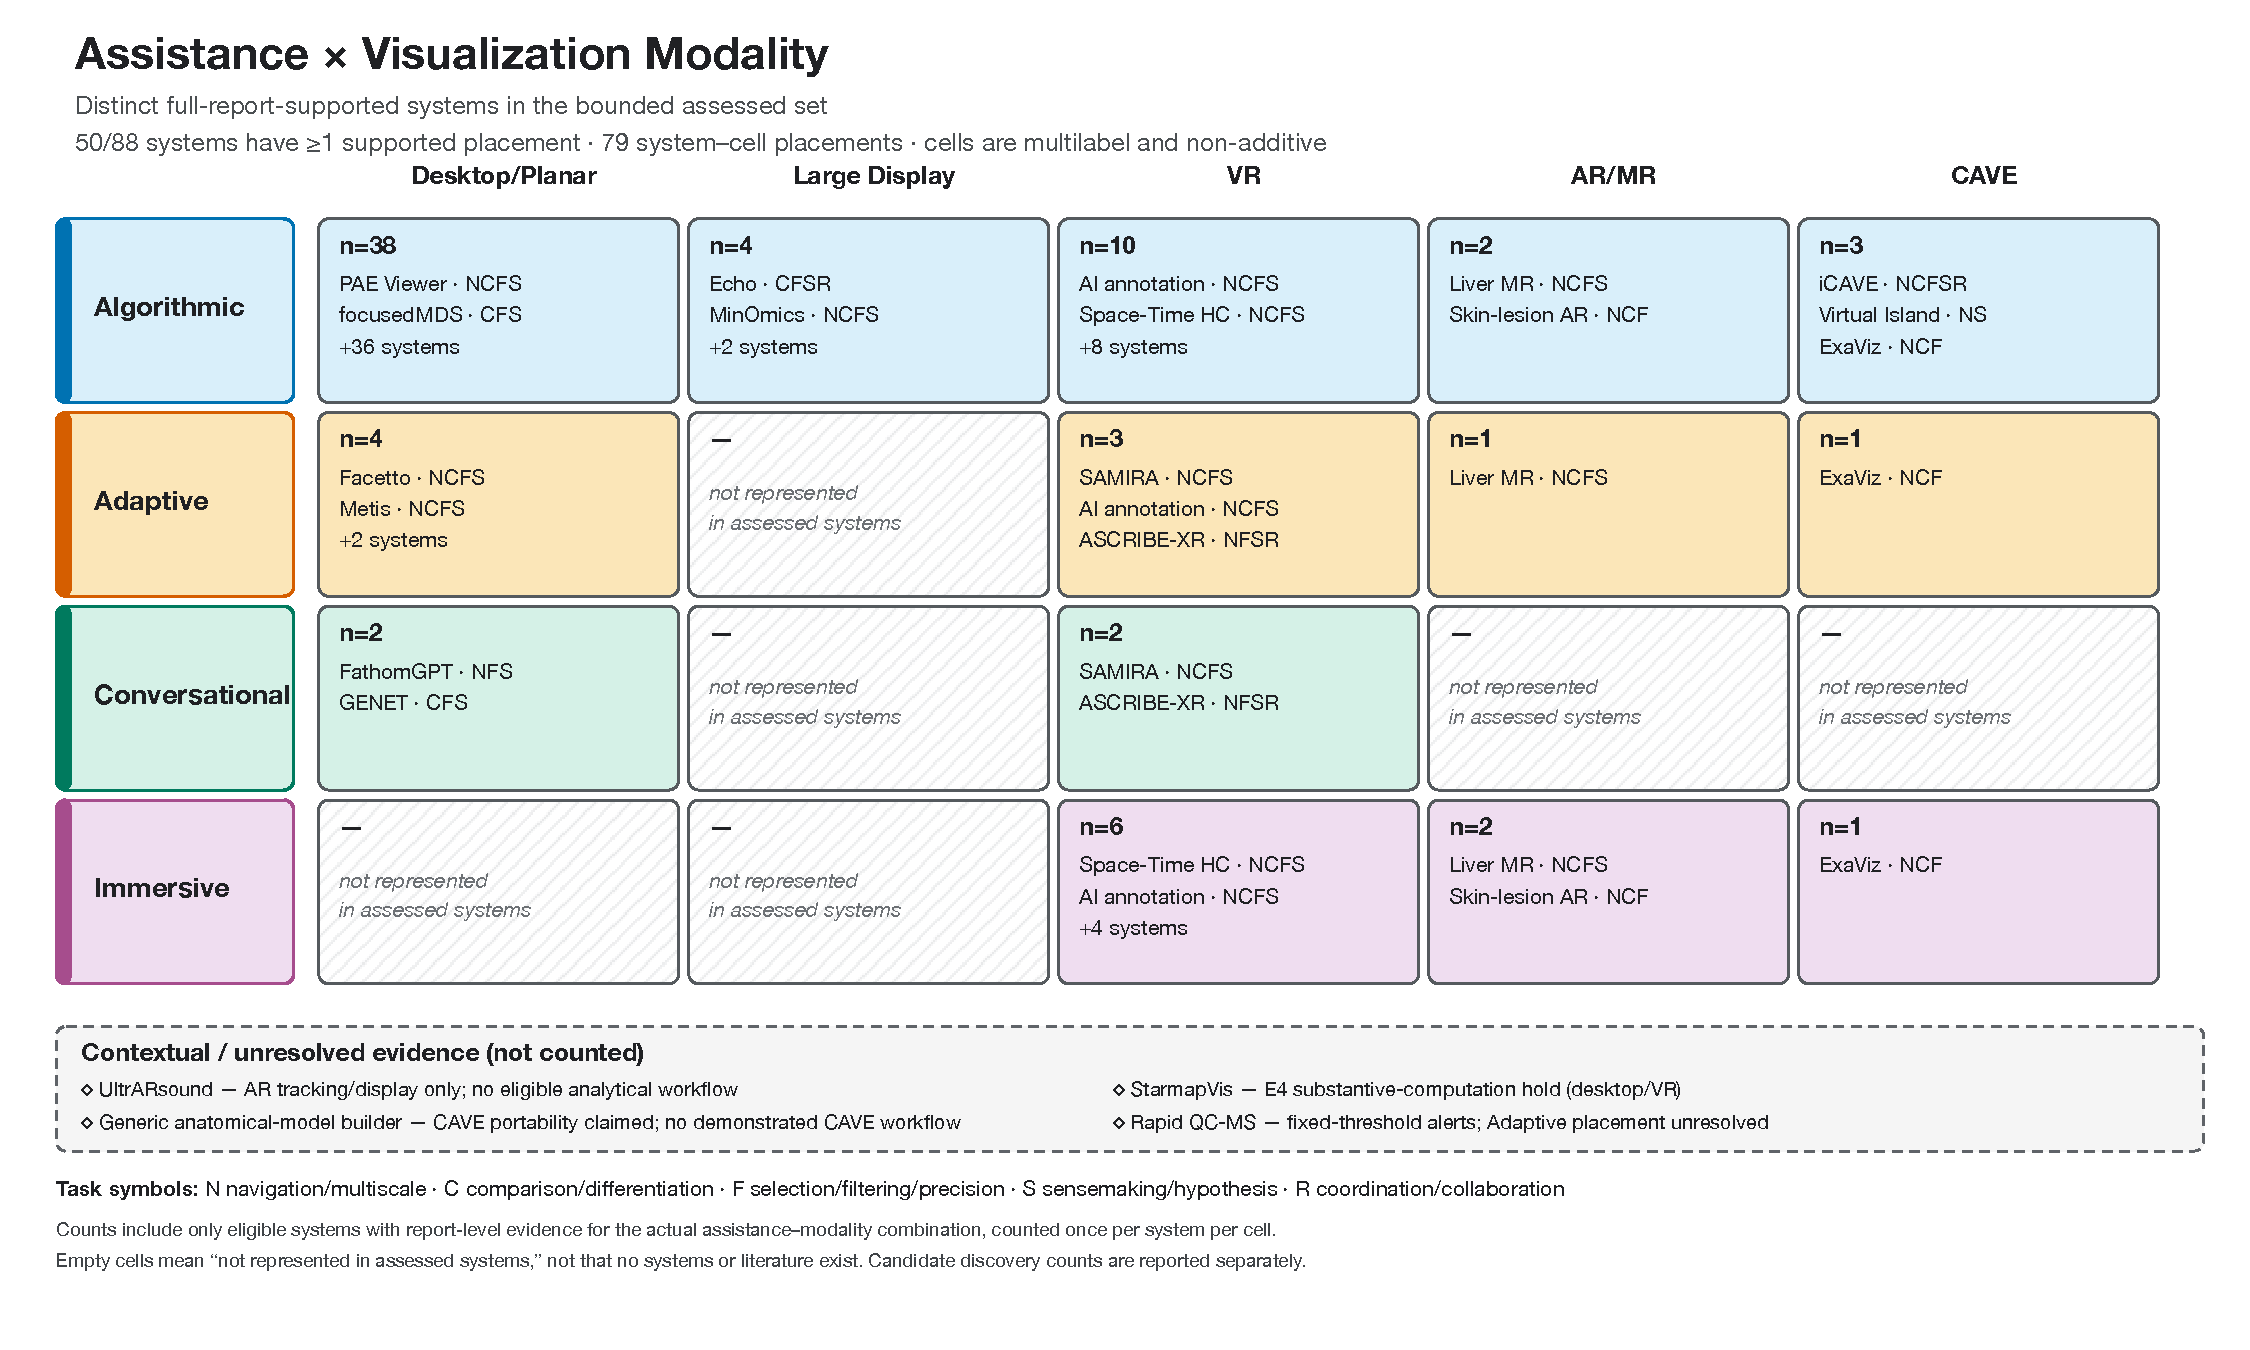
\includegraphics[width=\textwidth]{expanded_assistance_visualization_modality_map.pdf}
  \caption{Assistance × visualization modality map for the bounded cumulative assessed set. Counts denote distinct eligible systems with report-level evidence for the actual assistance–modality combination, counted once per system per cell; 50 of 88 considered systems have at least one supported placement, yielding 79 non-additive system–cell placements. Systems may occupy multiple cells when each relationship is separately supported. Task symbols indicate Navigation and Multiscale Orientation (N), Comparison and Differentiation (C), Selection, Filtering, and Precision Interaction (F), Sensemaking and Hypothesis Development (S), and Coordination and Collaborative Reasoning (R). Dashed examples are contextual or unresolved and are not counted. Empty cells mean “not represented in assessed systems,” not that no relevant systems or literature exist. Machine-coded candidate co-occurrences are discovery counts and are not encoded in the figure.}
  \label{fig:assistance-modality-map}
\end{figure*}
